% Figure 1 (fig:design): study design. No results are shown in this figure.
% Adapted from fig1_framework.tex. Drawn at the printed size: 18.19 cm = 7.16 in (full text width), so that
% \includegraphics[width=\textwidth] does not rescale it; the smallest type is 7 pt Helvetica.
% Panel a uses real images cropped from the pipeline's own example sheet (tiles/mri_*.png; brain MRI, TCGA-LGG).
% Panel b is drawn schematically (no colonoscopy video frame is stored in the repository).
% Build: pdflatex fig1_design.tex   (run in this folder; needs tiles/)
\documentclass[tikz,border=0pt]{standalone}
\usepackage{helvet}
\usepackage{sansmath}
\renewcommand{\familydefault}{\sfdefault}
\usetikzlibrary{arrows.meta,calc}
\definecolor{tblue}{HTML}{33669A}
\definecolor{tred}{HTML}{BB2E3F}
\definecolor{band}{HTML}{F3F4F6}
\definecolor{ink}{HTML}{1F1F1F}
\definecolor{muted}{HTML}{555555}
\definecolor{boxyellow}{HTML}{F2B705}
\definecolor{boxcyan}{HTML}{19C6E0}
\definecolor{mucosa}{HTML}{E08A6E}
\definecolor{mucosadark}{HTML}{9C4636}
\definecolor{mucosalight}{HTML}{F3B49C}
\definecolor{polyp}{HTML}{B8443A}
\hyphenpenalty=10000 \exhyphenpenalty=10000
\begin{document}
\sansmath
\begin{tikzpicture}[
  x=1cm, y=1cm,
  font=\fontsize{7}{8.6}\selectfont\color{ink},
  >={Stealth[length=4.2pt,width=3.6pt]},
  flow/.style={->, line width=0.8pt, draw=black!60},
  box/.style={draw=black!45, line width=0.4pt, fill=white, rounded corners=1.5pt},
  pnl/.style={font=\fontsize{9}{10}\selectfont\bfseries, anchor=base west},
  ttl/.style={font=\fontsize{8}{9.6}\selectfont\bfseries, anchor=base west},
  col/.style={font=\fontsize{7.5}{9}\selectfont\bfseries, anchor=base},
  desc/.style={font=\fontsize{7}{8.4}\selectfont, text=muted, anchor=north, align=center},
  ans/.style={font=\fontsize{8.5}{10}\selectfont\bfseries, anchor=base},
  hd/.style={font=\fontsize{7.5}{9}\selectfont\bfseries, anchor=north west, align=left},
  bd/.style={font=\fontsize{7}{8.6}\selectfont, anchor=north west, align=left},
]
\useasboundingbox (0,-0.24) rectangle (18.19,10.32);

% ================================================================= backgrounds of panels a and b
\fill[band, rounded corners=3pt] (0,4.40) rectangle (11.62,10.32);
\fill[band, rounded corners=3pt] (11.84,4.40) rectangle (18.19,10.32);

% ================================================================= panel a: matched views of one real case
\node[pnl] at (0.22,9.90) {a};
\node[ttl] at (0.62,9.90) {Matched views of one case};
\node[anchor=base west] at (0.24,9.42)
  {Question on every view: \textit{``Is there an abnormality in this brain MRI slice?''}};

\foreach \i/\t in {0/Original, 1/Lesion erased, 2/Control edit, 3/Lesion-free image} {
  \node[col] at (1.60+\i*2.8,8.92) {\t};
}
% tiles are 373 x 329 px (control: 374 x 329); trim = left bottom right top, in px, to crop the black margin
\node[inner sep=0pt, anchor=north west] at (0.35,8.74)
  {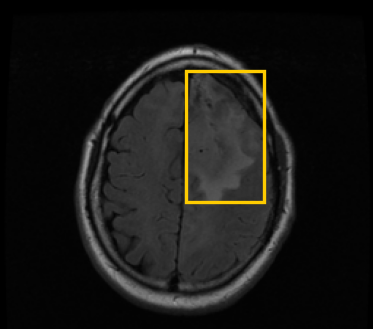
\includegraphics[width=2.5cm, trim=44 18 44 4, clip]{tiles/mri_orig.png}};
\node[inner sep=0pt, anchor=north west] at (3.15,8.74)
  {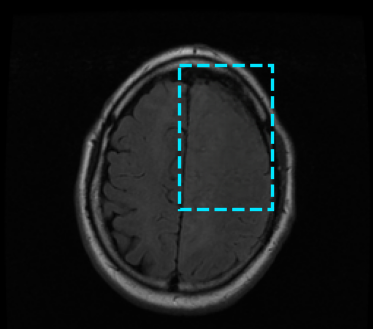
\includegraphics[width=2.5cm, trim=44 18 44 4, clip]{tiles/mri_erased.png}};
\node[inner sep=0pt, anchor=north west] at (5.95,8.74)
  {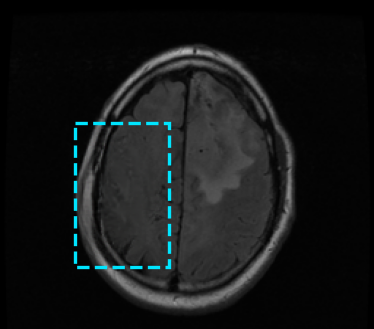
\includegraphics[width=2.5cm, trim=45 18 44 4, clip]{tiles/mri_control.png}};
\node[inner sep=0pt, anchor=north west] at (8.75,8.74)
  {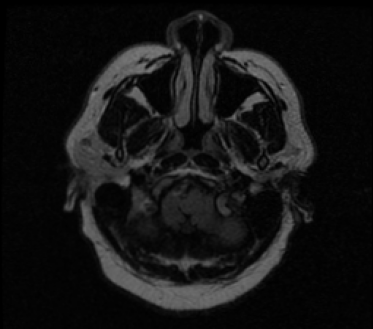
\includegraphics[width=2.5cm, trim=44 18 44 4, clip]{tiles/mri_free.png}};
% what is drawn on each view
\draw[boxyellow, line width=1.1pt] (0.50,5.75) -- (0.86,5.75);
\node[desc, anchor=north west] at (0.90,5.92) {expert lesion box};
\draw[boxcyan, line width=1.1pt, dash pattern=on 2.2pt off 1.4pt] (3.47,5.75) -- (3.87,5.75);
\node[desc, anchor=north west] at (3.91,5.92) {edited region};
\node[desc] at (7.20,5.92) {same shape and tool,\\elsewhere in the image};
\node[desc] at (10.00,5.92) {no lesion, no edit};
% expected answers
\draw[black!30, line width=0.4pt] (0.35,5.07) -- (3.25,5.07);
\draw[black!30, line width=0.4pt] (8.35,5.07) -- (11.25,5.07);
\node[anchor=base, text=muted] at (5.80,4.995) {Answer of a model that uses the image};
\node[ans, text=tblue] at (1.60,4.62) {present};
\node[ans, text=tred]  at (4.40,4.62) {absent};
\node[ans, text=tblue] at (7.20,4.62) {present};
\node[ans, text=tred]  at (10.00,4.62) {absent};

% ================================================================= panel b: unedited pair from one video
\node[pnl] at (12.06,9.90) {b};
\node[ttl] at (12.46,9.90) {Unedited pair from one video};
\node[anchor=base west] at (12.08,9.42) {Question: \textit{``Is there a polyp in this image?''}};

% film strip: nine frames of one colonoscopy video; the polyp is in view in frames 2 to 4
\fill[black!78, rounded corners=1.2pt] (12.24,8.60) rectangle (17.79,9.18);
\foreach \k in {0,...,8} {
  \fill[mucosa] (12.34+\k*0.6,8.69) rectangle ++(0.5,0.40);
}
\foreach \k in {1,2,3} {
  \fill[polyp] (12.34+\k*0.6+0.30,8.85) circle (0.075);
}
\draw[white, line width=1.0pt] (12.34+2*0.6,8.69) rectangle ++(0.5,0.40);
\draw[white, line width=1.0pt] (12.34+6*0.6,8.69) rectangle ++(0.5,0.40);
\draw[black!55, line width=0.5pt] (13.79,8.60) -- (13.52,8.48);
\draw[black!55, line width=0.5pt] (16.19,8.60) -- (16.52,8.48);

\node[col] at (13.52,8.25) {Lesion frame};
\node[col] at (16.52,8.25) {Lesion-free frame};

% enlarged frames (schematic endoscope views)
\foreach \cx/\haspolyp in {13.52/1, 16.52/0} {
  \fill[black] (\cx-1.25,6.22) rectangle (\cx+1.25,8.07);
  \begin{scope}
    \clip (\cx,7.145) circle (0.86);
    \shade[inner color=mucosadark!85!black, outer color=mucosa] (\cx-0.23,7.32) circle (1.35);
    \draw[mucosalight, line width=1.5pt, opacity=0.75] (\cx-0.23,7.32) ++(200:0.57) arc (200:340:0.57);
    \draw[mucosalight, line width=1.2pt, opacity=0.65] (\cx-0.23,7.32) ++(20:0.46) arc (20:150:0.46);
    \draw[mucosalight, line width=1.7pt, opacity=0.70] (\cx-0.23,7.32) ++(215:0.90) arc (215:330:0.90);
    \draw[mucosalight, line width=1.3pt, opacity=0.60] (\cx-0.23,7.32) ++(5:0.85) arc (5:120:0.85);
    \ifnum\haspolyp=1
      \shade[ball color=polyp] (\cx+0.37,6.83) ellipse (0.25 and 0.21);
    \fi
  \end{scope}
  \ifnum\haspolyp=1
    \draw[boxyellow, line width=1.1pt] (\cx+0.05,6.55) rectangle (\cx+0.69,7.11);
  \fi
}
\draw[boxyellow, line width=1.1pt] (12.52,5.92) -- (12.88,5.92);
\node[desc, anchor=north west] at (12.92,6.09) {annotated polyp};
\node[desc] at (16.52,6.09) {same video, no polyp};
\node[desc] at (15.02,5.76) {no image is edited; frames drawn schematically};
% expected answers
\node[anchor=base, text=muted] at (15.02,4.995) {Answer of a model that uses the image};
\node[ans, text=tblue] at (13.52,4.62) {present};
\node[ans, text=tred]  at (16.52,4.62) {absent};

% ================================================================= panel c: study flow
\node[pnl] at (0.22,3.86) {c};
\node[ttl] at (0.62,3.86) {Study flow};

\def\ytop{3.58}\def\ybot{-0.22}
% box 1: public datasets
\draw[box] (0.01,\ybot) rectangle (2.56,\ytop);
\node[hd, text width=2.3cm] at (0.10,3.48) {Public\\datasets};
\node[bd, text width=2.30cm] at (0.10,2.72)
  {Images with expert lesion masks: MRI, CT, ultrasound, X-ray, colonoscopy.\\[3pt]
   Colonoscopy videos with polyp boxes on the frames.};
% box 2: automated views and quality checks
\draw[box] (2.94,\ybot) rectangle (6.34,\ytop);
\node[hd, text width=3.2cm] at (3.03,3.48) {Automated views and\\quality checks};
\node[bd, text width=3.16cm] at (3.03,2.72)
  {Per case: erasure, control edit and a lesion-free image (a). Per video: one frame pair (b).\\[3pt]
   The control edit changes no lesion pixel; no near-copies across splits; two editing tools kept out of
   training.};
% box 3: agent loop
\draw[box] (6.72,\ybot) rectangle (10.12,\ytop);
\node[hd, text width=3.2cm] at (6.81,3.48) {Same agent loop\\for every model};
\node[bd, text width=3.16cm] at (6.81,2.72)
  {One image and the question. The model may zoom or adjust contrast (at most 3 tool calls), then answers
   present or absent, or refers.\\[3pt]
   Same prompt, tools and images for all models.};
% box 4: measures
\draw[box] (10.50,\ybot) rectangle (15.40,\ytop);
\node[hd, text width=4.6cm] at (10.59,3.48) {Measures};
\node[bd, text width=4.66cm] at (10.59,3.06)
  {Evidence sensitivity gap, from (a):\\
   \hspace*{0.7em}ESG $=$ $D$(\textcolor{tred}{erased}) $-$ $D$(\textcolor{tblue}{control edit})\\[2pt]
   Natural ESG, from (b):\\
   \hspace*{0.7em}$D$(\textcolor{tred}{lesion-free frame}) $-$ $D$(\textcolor{tblue}{lesion frame})\\[2pt]
   $D$: share answered absent or referred.\\
   Both gaps are 0 if the image is ignored.\\[3pt]
   Also: erased-lesion claims, lesion-free\\claims, lesion images correct, net utility.};
% box 5: reader assessment
\draw[box] (15.78,\ybot) rectangle (18.18,\ytop);
\node[hd, text width=2.2cm] at (15.87,3.48) {Reader\\assessment};
\node[bd, text width=2.10cm] at (15.87,2.72)
  {Specialist readers, not told which images are edited, judge a sample of test images: edited or not?
   finding present or not?};
% arrows between boxes
\foreach \xa/\xb in {2.60/2.90, 6.38/6.68, 10.16/10.46, 15.44/15.74} {
  \draw[flow] (\xa,1.68) -- (\xb,1.68);
}
\end{tikzpicture}
\end{document}
